\documentclass[a4paper, 10pt, conference]{ieeeconf}
\IEEEoverridecommandlockouts  
\overrideIEEEmargins     
\bibliographystyle{IEEEtran}
\pdfminorversion=4


\usepackage{cite}
%\usepackage{mathptmx}       % selects Times Roman as basic font
\usepackage{helvet}         % selects Helvetica as sans-serif font
\usepackage{courier}        % selects Courier as typewriter font
\usepackage{type1cm}        % activate if the above 3 fonts are
                            % not available on your system
%
\usepackage{makeidx}         % allows index generation
\usepackage{graphicx}        % standard LaTeX graphics tool
%                             % when including figure files
\usepackage{multicol}        % used for the two-column index
\usepackage{times}
\usepackage{xfrac}
%\usepackage{mathabx}
\usepackage[thref]{ntheorem} % Uncomment this in Windows version
\usepackage{amsfonts}%
\usepackage{amssymb}%
\usepackage{color}
%\usepackage{import}
\usepackage{graphicx,psfrag}
\usepackage{float}
\usepackage[cmex10]{amsmath}
%\usepackage{amsthm} % Comment this in Windows version
\newtheorem{theorem}{Theorem}
\newtheorem{lemma}{Lemma}
\newtheorem*{remark}{Remark}
\newcommand{\jo}{(e^{-j\omega})}
\newcommand{\jok}{(e^{-j\omega_k})}
\newcommand{\jro}{(e^{-j\omega},\rho)}
\newcommand{\jrok}{(e^{-j\omega_k},\rho)}
%\renewcommand{\IEEEQED}{\IEEEQEDopen}
\renewcommand{\vec}[1]{\mathbf{#1}}
\newcommand{\hilight}[1]{\colorbox{yellow}{#1}}
%\DeclareRobustCommand*{\IEEEauthorrefmark}[1]{%
  %\raisebox{0pt}[0pt][0pt]{\textsuperscript{\footnotesize\ensuremath{#1}}}}

\title{\LARGE \bf A Data-Driven Approach in Designing RST Controllers with $H_{\infty}$ performance via Convex Optimization}

\author{Achille Nicoletti, Zlatko Emedi and Alireza Karimi % <-this % stops a space
\thanks{Automatic Control Laboratory,
Ecole Polytechnique F\'{e}d\'{e}rale de Lausanne (EPFL),
1015 Lausanne, Switzerland}%
%\thanks{$^{3}$ {\tt\small achille.nicoletti@epfl.ch}}%
%\thanks{$^{4}$ {\tt\small michele.martino@cern.ch}}%
\thanks{Corresponding author: {\tt\small alireza.karimi@epfl.ch}}%
}

\begin{document}

\maketitle
\thispagestyle{empty}
\pagestyle{empty}

\begin{abstract}
In this paper, a new method for designing robust fixed-order $\mathcal{H}_{\infty}$ discrete-time controllers is presented. The controller structure is a two-degree of freedom polynomial controller of the RST-type. A data-driven approach is implemented for the design process in order to capture the unmodeled dynamics that may exist with parametric models. The $\mathcal{H}_{\infty}$ robust performance condition can be represented by a set of convex constraints with respect to the parameters of the RST controllers. A convex optimization algorithm can then be implemented to obtain these parameters. The proposed method is applied to a multi-axis torsional system where the goal is to control the position of the disks with variable inertias.
\end{abstract}


\section{Introduction}
In many of today's complex industrial applications, it is difficult to model a process with extreme precision. For such processes, a high-order model is typically required to capture the dynamics of a system; however, high order models lead to high order controllers with numerical implementation problems.  Therefore, in practice, low-order models are preferred in order to simplify the controller design process. However, low-order models possess unmodeled dynamics that can hinder the performance of a controller. Robust controller design methods use the uncertainty models as weighting filters to ensure the stability and performance of the closed-loop system. This in turn increases the controller order which is equal to the order of the plant model and the uncertainty weighting filter. In data-driven methods, the plant model is represented by a set of data; thus there are no unmodeled dynamics and the controller order can be chosen independently of the plant model complexity.  The data-driven approach can be realized in two manners: using time-domain or frequency-domain data. In this paper, the frequency-domain approach will be utilized for the controller design scheme.

The field of frequency-domain controller design techniques continues to spark the interest of many researchers. In \cite{KNN13}, a controller is designed in the frequency-domain by considering a least-squares optimization approach; however, in this method, it is not evident on how to predefine the structure of a stabilizing controller. A data-driven design method that guarantees the stability of a closed-loop system by setting gain and phase margin constraints in the Nyquist diagram has been addressed in \cite{Sae13}. Despite the simplicity and advantages of this method, it cannot be applied to unstable plants. Moreover, the constraints are conservative and may lead to a controller that inhibits the system performance. %A learning algorithm to design a controller in the frequency-domain was examined in \cite{LWZ10}, though it is not clear how the robustness margins are defined. 
A robust frequency-domain control design method has been established in \cite{KNDB13}; this method, however, requires a solution to a non-linear optimization problem. 

Robust control methods are continually addressed within the control system community. Many research papers and books have been devoted to developing new algorithms in designing robust controllers that reduce the conservatism associated with uncertainty modeling. Robust controller design methods belonging to the $\mathcal{H}_{\infty}$ control framework minimizes the $\mathcal{H}_{\infty}$ norm of a weighted closed-loop sensitivity function. An $\mathcal{H}_{\infty}$ loop-shaping method to design stabilizing controllers has been examined in \cite{YYH13}. However, a non-convex optimization algorithm is required to obtain a solution. Generally, it is desired to acquire a convex optimization problem since convex problems are computationally tractable. A convex approximation of the $\mathcal{H}_\infty$ criterion has been discussed in \cite{KG10} and \cite{KGL08} where convex constraints are imposed on the Nyquist diagram. The controller is linearly parameterized (the denominator is fixed) and a desired open loop transfer function is used to convexify the $\mathcal{H}_{\infty}$ constraints.  An extension to this method has been presented in \cite{KZ04}, where a single-input-single-output (SISO) controller is represented in a rational form (and thus allowing the numerator and denominator of a controller to be optimized separately). This method gives the necessary and sufficient conditions for the existence of a robust controller for systems represented by a frequency response function.

The RST controller structure is an effective discrete-time two-degree of freedom polynomial controller where the tracking and regulation characteristics of a closed-loop system can be formulated independently \cite{LZ06}. %The general $RST$ controller structure is shown in Fig.\ref{fig:rst_simp}. 
Various methods and applications of the RST controller design methodology have been addressed in \cite{BTA14}, \cite{LHM10}, \cite{KH11}, and \cite{MBH13}. However, in these previous applications, the controllers were devised based on the knowledge of the dynamic model of the physical system. A frequency domain approach in designing the RST controllers has been discussed in \cite{GKL11}. In this approach, a convex optimization algorithm was formulated by considering a convex approximation of the $\mathcal{H}_{\infty}$ criterion. However, in order to preserve convexity, this method required one of the controller terms ($R$) to be fixed a priori. 

%\begin{figure}
%\centering
%\resizebox{1.0\columnwidth}{!}{\input{rst_simp.eps_tex}}
%\caption{RST controller structure}
%\label{fig:rst_simp}
%\end{figure}

The proposed method in this paper is an extension of \cite{GKL11} and \cite{KZ04}, where an RST controller will be designed by formulating a convex optimization problem in the frequency domain. In \cite{GKL11}, the controller $R$ was fixed with an integrator\footnote{Note that the variable names for $R$ and $S$ are interchanged in \cite{GKL11}}, while $S$ and $T$ where linearly parameterized. However, with the methodology presented in this paper, the $R$, $S$ and $T$ controllers can each be linearly parameterized, and thus introduces more degrees of freedom which improves the $\mathcal{H}_{\infty}$ performance. Moreover, new convex constraints are imposed in order to guarantee that the closed-loop system remains stable while attaining the desired tracking performance without the need to specify a desired open-loop transfer function.
 
This paper is organized as follows: In section (\ref{sec:2}), the class of models, controllers and control objectives are defined. Section (\ref{sec:3}) will discuss the control design methodology and stability conditions of the proposed method for the RST controller structure. Convex conditions will be formulated based on the $\mathcal{H}_{\infty}$ criterion. Section (\ref{sec:4}) will demonstrate the effectiveness of the method by applying the proposed design scheme to a multi-axis torsional system. Finally the concluding remarks are given in Section (\ref{sec:5}).

\textbf{Notation}: In order to avoid the risk of any confusion, the notation for the symbols employed in this paper will be defined here.
\begin{align*}
\mathbb{R} &: \ \mbox{the set of all real numbers.} \\
\mathbb{Z} &: \ \mbox{the set of all positive integers including zero.} \\
\mathcal{R}e\{\cdot \} &: \ \mbox{the real part of a complex variable.} \\
\mathcal{I}m\{\cdot \} &: \ \mbox{the imaginary part of a complex variable.} \\
a^{\top} &: \ \mbox{the transpose of the vector }a. \\
z &: \ \parbox[t]{18em}{variable used to represent the complex frequency domain of discrete-time systems.} \\
s &: \ \parbox[t]{18em}{variable used to represent the complex frequency domain of continuous-time systems.}
\end{align*} 
%\section{Notation and Preliminaries}
%Due to the nature of the equations asserted in this paper, it will be convenient express certain equations in a compact manner. A cascade of $q$ frequency response functions $A_1(e^{-j\omega})A_2(e^{-j\omega}) \cdots A_q(e^{-j\omega})$ will be denoted as $[A_1A_2 \cdots A_q](e^{-j\omega})$. 


\section{Problem Formulation}
\label{sec:2}


\subsection{Class of models}
\label{sec:21}
Let us begin by considering the frequency response function (FRF) of a discrete-time SISO plant given as
\begin{equation}\label{eq:G_frf}
G(e^{-j\omega}) = N(e^{-j\omega}) M^{-1}(e^{-j\omega}), \qquad \forall \omega \in \Omega
\end{equation}
where $\Omega \in [0,\pi]$. $N(e^{-j\omega})$ and $M(e^{-j\omega})$ must be FRF's of bounded analytic functions outside the unit circle. For stable plants, a trivial choice is $N(e^{-j\omega})=G(e^{-j\omega})$ and $M(e^{-j\omega})=1$. For unstable plants, $N(e^{-j\omega})$ and $M(e^{-j\omega})$ can be obtained, in a data-driven setting, by considering the acquired data of a closed-loop system with a stabilizing controller. If $N(e^{-j\omega})$ represents the FRF of the transfer function from the reference input to the output, and $M(e^{-j\omega})$ represents the FRF of the transfer function from the reference input to the controller output, then the FRF of the plant model can be obtained as asserted in (\ref{eq:G_frf}).
%A discussion on how to formulate $N(e^{-j\omega})$ and $M(e^{-j\omega})$ for systems that are not BIBO stable can be found in \cite{KZ04}. 

In general, a set $\mathcal{G}$ that represents a plant model containing $k$ FRF models can be defined:
\begin{equation}
\mathcal{G} = \{G_i(e^{-j\omega}); \quad i=1,\ldots,k; \quad \forall \omega \in \Omega\}
\end{equation} 
These FRF's can be determined by considering the frequency response of a parametric model or from a set of input/output data. For simplicity, one model from the set $\mathcal{G}$ will be considered, and the subscript $i$ will be omitted. However, in general, the design procedures outlined in this paper can be applied to the multi-model case. In section (\ref{sec:4}), the proposed method is applied on a torsional apparatus with multi-model uncertainty. 

\subsection{Class of controllers}
The controller structure that will be considered will be of the RST-type, as shown in Fig.\ref{fig:rst}. The RST controllers are linearly parameterized in the variables $r_k$, $s_k$, and $t_k$; they are each polynomials in $z$ which can be expressed as:
\begin{alignat}{2}
R(z^{-1}) &= r_0 + r_1z^{-1} + \cdots + r_{n_r}z^{-n_r} \label{eq:Rc}\\
S(z^{-1}) &= 1 + s_1z^{-1} + \cdots + s_{n_s}z^{-n_s} \label{eq:Sc}\\
T(z^{-1}) &= t_0 + t_1z^{-1} + \cdots + t_{n_t}z^{-n_t} \label{eq:Tc}
\end{alignat}
where $\{n_r,n_s,n_t\} \in \mathbb{Z}$. These controllers can also be represented in vector form as $R(z^{-1},\rho)=\rho_R^\top \phi_R(z^{-1})$, $S(z^{-1},\rho)=\rho_S^\top \phi_S(z^{-1})$ and $T(z^{-1},\rho)=\rho_T^\top \phi_T(z^{-1})$, where 
\begin{alignat}{4}
\rho_R^\top &= [r_0,r_1,\ldots,r_{n_r}]; &&\quad \phi_R^\top(z^{-1}) &&&= [1,z^{-1},\ldots,z^{-n_r}]\\
\rho_S^\top &= [1,s_1,\ldots,s_{n_s}]; &&\quad \phi_S^\top(z^{-1}) &&&= [1,z^{-1},\ldots,z^{-n_s}]\\
\rho_T^\top &= [t_0,t_1,\ldots,t_{n_t}];  &&\quad \phi_T^\top(z^{-1}) &&&= [1,z^{-1},\ldots,z^{-n_t}]
\end{alignat}
%The purpose of parameterizing the controllers in this manner will become apparent in subsequent sections.
%For notation purposes, the dependency on the discrete-time frequency variable $z^{-1}$ will be omitted, and the dependency on the controller parameter $\rho$ will remain. 
\begin{figure}
\centering
\resizebox{1.0\columnwidth}{!}{\input{rst.eps_tex}}
\caption{RST controller structure}
\label{fig:rst}
\end{figure}

\subsection{Process Definitions}
\label{sec:23}
Since the design techniques introduced in this paper belong to the $\mathcal{H}_{\infty}$ framework, it is  appropriate to consider the various sensitivity functions associated with the controller structure shown in Fig.~\ref{fig:rst}. Some of the sensitivity functions for this process can be asserted as follows:
\begin{eqnarray}
\mathcal{S}_0(z^{-1},\rho)&=&\frac{M(z^{-1})S(z^{-1},\rho)}{\psi(z^{-1},\rho)}  \label{eq:S0}\\
\mathcal{S}_i(z^{-1},\rho)&=&\frac{N(z^{-1})S(z^{-1},\rho)}{\psi(z^{-1},\rho)} \\
\mathcal{T}(z^{-1},\rho)&=&\frac{N(z^{-1})T(z^{-1},\rho)}{\psi(z^{-1},\rho)} \label{eq:T} \\
\mathcal{U}(z^{-1},\rho)&=&\frac{M(z^{-1})T(z^{-1},\rho)}{\psi(z^{-1},\rho)} \label{eq:U}\\
\mathcal{V}(z^{-1},\rho)&=& -\frac{N(z^{-1})R(z^{-1},\rho)}{\psi(z^{-1},\rho)} \\
\mathcal{E}(z^{-1},\rho)&=&\frac{\psi(z^{-1},\rho) - N(z^{-1})T(z^{-1},\rho)}{\psi(z^{-1},\rho)} \label{eq:err}
\end{eqnarray}
where $\psi(z^{-1},\rho) = M(z^{-1})S(z^{-1},\rho)+N(z^{-1})R(z^{-1},\rho)$ and $\mathcal{S}_0(z^{-1},\rho)$ is the transfer function between $d_o$ and $y$, $\mathcal{S}_i(z^{-1},\rho)$ is the transfer function between $d_i$ and $y$, $\mathcal{T}(z^{-1},\rho)$ is the transfer function between $r$ and $y$, $\mathcal{U}(z^{-1},\rho)$ is the transfer function between $r$ and $u$, $\mathcal{V}(z^{-1},\rho)$ is the transfer function between $v$ and $y$, and $\mathcal{E}(z^{-1},\rho)$ is the transfer function between $r$ and the tracking error signal $r-y$. Note that all of the sensitivity functions are stable if the zeros of $\psi(z^{-1},\rho)$ lie within the unit circle. Based on the internal model principle, the controller may contain the disturbance model to achieve a zero steady-state error. Therefore, the controllers may be pre-multiplied with any arbitrary function that actualizes the desired performance. For example, if it is desired to reject a step disturbance at the output, then $S(z^{-1},\rho)$ can be pre-multiplied with $(1-z^{-1})$ (which represents the integral action of the controller). 


\section{$\mathcal{H}_{\infty}$ Performance via Convex Optimization}
\label{sec:3}
\subsection{Preliminary Design Specifications}
Suppose that it is desired to shape a particular sensitivity function. Consider, for example, the sensitivity function from $d_o$ to $y$, expressed as $\mathcal{S}_0(z^{-1},\rho)$. Given a stable weighting filter $W_1$ with a bounded infinity norm, a necessary and sufficient condition for achieving nominal performance is given by \cite{Zho98}:
\begin{equation} \label{eq:inf1}
\| W_1\mathcal{S}_0 \|_{\infty}<\gamma
\end{equation}
where $\{ \gamma \in \mathbb{R} \mid \gamma > 0 \}$. In general, this condition can be extended to any of the sensitivity functions asserted in section (\ref{sec:23}). This condition can also be expressed as follows:
\begin{equation} \label{eq:inf_f}
 |W_1(e^{-j\omega}) \mathcal{S}_0(e^{-j\omega},\rho)| < \gamma; \quad \forall \omega \in \Omega
\end{equation}
For notation purposes, the dependency in $e^{-j\omega}$ will be omitted, and will only be reiterated when deemed necessary. The dependency on $\rho$ will continue to be highlighted. Notice that (\ref{eq:inf_f}) can also be written as
\begin{equation} \label{eq:circle}
\gamma^{-1}|W_1MS(\rho)| < |\psi(\rho)| ; \quad \forall \omega \in \Omega
\end{equation}
where $\psi(\rho) = MS(\rho) + NR(\rho)$. It is desired to minimize the upper bound $\gamma$ such that the $\mathcal{H}_{\infty}$ performance condition is satisfied. %This phenomenon is known as \textit{optimal $\mathcal{H}_{\infty}$ control}. 
Therefore, the following optimization problem can be considered:
\begin{equation} \label{eq:min1}
\begin{aligned}
& \underset{ \{\rho_R,\rho_S,\rho_T\} \in \mathbb{R}}{\text{minimize}}
& & \gamma  \\
& \text{subject to:} & & \gamma^{-1} |W_1MS(\rho)| < |\psi(\rho)|  \\ 
& & & \forall \omega \in \Omega
\end{aligned}
\end{equation}
Notice that (\ref{eq:min1}) is both a non-linear and non-convex optimization problem. 
\begin{remark}
Note that the controller $T(z^{-1},\rho)$ was not considered in the optimization problem (\ref{eq:min1}) since $\mathcal{S}_0(z^{-1},\rho)$ is independent of $T(z^{-1},\rho)$. One of the benefits of implementing the RST controller is that the tracking performance can be specified independently from the regulation requirements, and thus the controller $T(z^{-1},\rho)$ can be designed once $R(z^{-1},\rho)$ and $S(z^{-1},\rho)$ have been obtained. If tracking performance is crucial for the design, one may consider minimizing $\gamma$ for $\|W_2\mathcal{E} \| _{\infty}<\gamma$, where $W_2$ is also a stable transfer function with a bounded infinity norm. 
\end{remark}


\begin{figure}
\centering
\resizebox{0.8\columnwidth}{!}{\input{nxmy2.eps_tex}}
\caption{The $\mathcal{H}_{\infty}$ constraint in (\ref{eq:inf1}) can be represented as a circle in the complex plane. The constraint ensures that the circle will never encircle the origin for any frequency point in $\Omega$.}
\label{fig:circle}
\end{figure}
Consider a circle in the complex plane which is centered at $MS(\rho) + NR(\rho)$ and has radius $\gamma^{-1}|W_1MS(\rho)|$. The constraint in (\ref{eq:circle}) ensures that for any frequency point in $\Omega$, the circle associated with this frequency point will not encircle the origin. Figure \ref{fig:circle} displays the graphical interpretation of this condition. According to \cite{KZ04}, for each $\omega \in \Omega$ there exists a complex number $f(e^{-j\omega})$ which can rotate the disk in Fig.~\ref{fig:circle} such that it lays on the right hand side of the imaginary axis:
\begin{equation}\label{eq:real}
\mathcal{R}e\{Z(\rho) f(e^{-j\omega}) \} > 0; \quad \forall \omega \in \Omega
\end{equation}
where $Z(\rho) = \psi(\rho) - \gamma^{-1} |W_1MS(\rho)|$. In \cite{RM94}, it is shown that $f(e^{-j\omega})$ can be approximated arbitrarily well by the frequency response of a finite order transfer function if and only if $$[\psi(\rho) - \gamma_0^{-1}|W_1MS(\rho)|]^{-1}$$ is analytic in the right half plane for all $\gamma_0 > \gamma$. Based on (\ref{eq:real}) and on the results established in \cite{KZ04}, the following theorem can be formulated:
\begin{theorem}
Given $\gamma > 0$,  the performance criterion in (\ref{eq:inf1}) is satisfied if and only if there exist polynomials $R(z^{-1},\rho)$ and $S(z^{-1},\rho)$ such that
\begin{equation}
\begin{aligned} \label{eq:con1}
\gamma^{-1} |W_1MS(\rho)| < \mathcal{R}e\{\psi(\rho) \} \qquad 
\forall \omega \in \Omega 
\end{aligned}
\end{equation}
where $\psi(\rho) = MS(\rho) + NR(\rho)$.
\end{theorem}
\begin{proof}
The proof of a similar theorem has been formally documented in \cite{KZ04}\footnote{This proof was established by assuming a unity feedback system with a rational controller structure $K = XY^{-1}$ in the feedforward loop. For the RST controller structure used in this paper, the controller $R$ is equivalent to $X$ and $S$ is equivalent to $Y$.}.
\end{proof}




\iffalse
\begin{proof}
The proof of a similar theorem has been formally documented in \cite{KZ04}\footnote{This proof was established by assuming a unity feedback system with a rational controller structure $K = XY^{-1}$ in the feedforward loop. For the RST controller structure used in this paper, the controller $R$ is equivalent to $X$ and $S$ is equivalent to $Y$.}. By substituting the FRF of (\ref{eq:S0}) into (\ref{eq:inf_f}), the $\mathcal{H}_{\infty}$ constraint can be expressed as follows:
\begin{equation}
\begin{aligned}
\gamma^{-1} |W_1MS(\rho)| < |\psi(\rho) |& \\
\forall \omega \in \Omega &
\end{aligned}
\end{equation}
However, since $\mathcal{R}e\{\psi(\rho) \} \leq |\psi(\rho) |$ (i.e., the real part of a complex number is less than or equal to its magnitude), then the resulting constraint can be expressed as asserted in (\ref{eq:con1}).
\end{proof}
\fi





%%% Part about tracking a ramp
In certain design strategies, it may sometimes be desired to track different reference signals with no steady-state error, such as a step or a ramp input. For the torsional system that will be addressed in this paper, it will be desired to track a step input. Minimization of the error sensitivity function is a soft constraint, and may not lead to the ideal tracking performance. Therefore it is advantageous to consider conditions that ensure proper tracking of a step input by imposing hard convex constraints. Note that in an RST structure, the existence of an integrator in the open-loop transfer function does not guarantee a zero steady-state error for tracking a step input. The necessary and sufficient condition for a zero steady-state error is recalled in the following lemma. 

\begin{lemma}
Suppose that the reference signal is a step function given as $r(z^{-1}) = A(1-z^{-1})^{-1}$, where $A$ is the amplitude of the step function. Additionally, suppose that the controller $S(z^{-1},\rho)$ possesses an integrator (i.e., $S(z^{-1},\rho) = (1-z^{-1}) S^{\prime}(z^{-1},\rho)$, where $S^{\prime}(z^{-1},\rho)$ is linearly parameterized). A necessary and sufficient condition to obtain a zero steady-state error for a step input is
\begin{align} \label{eq:step_con}
R(1,\rho) = T(1,\rho) \neq 0
\end{align}
\end{lemma}

\begin{proof}
The proof for this condition can be established by using the final value theorem. For perfect tracking of an arbitrary reference signal $r(k)$, it is required that $\lim_{k \to \infty} [r(k)-y(k)] = 0$, or
\begin{equation}
\lim_{z \to 1}(1-z^{-1})r(z^{-1})[1-\mathcal{T}(z^{-1},\rho)] = 0
\end{equation}
For a step input, the condition for achieving a zero steady-state error can be expressed as
\begin{equation} \label{eq:lim1}
\lim_{z \to 1} [1-\mathcal{T}(z^{-1},\rho)] = 0 
\end{equation}
By substituting (\ref{eq:T}) into (\ref{eq:lim1}) (and noting that $S(z^{-1},\rho) = (1-z^{-1}) S^{\prime}(z^{-1},\rho)$), one can arrive to the following condition:
\begin{eqnarray} \label{eq:limf}
\lim_{z \to 1} \frac{N(z^{-1})[R(z^{-1},\rho) - T(z^{-1},\rho)]}{M(z^{-1})S(z^{-1},\rho) + N(z^{-1})R(z^{-1},\rho)} \nonumber\\
 = \frac{R(1,\rho) - T(1,\rho)}{R(1,\rho)} = 0
\end{eqnarray} 
which evidently leads to the  condition asserted in (\ref{eq:step_con}).
\end{proof}


\subsection{Convex Optimization via Semi-Definite Programming}
Suppose that it is desired to achieve proper tracking performance and zero steady-state error for a step reference input. Moreover, it is desired that the sensitivity function $\mathcal{U}(z^{-1},\rho)$ in (\ref{eq:U}) be shaped to limit the control efforts. As a result, the infinity norm of $W_2\mathcal{E}$ and $W_3\mathcal{U}$ should be minimized where $W_2$ is a lowpass filter with a cut off frequency close to the desired bandwidth and $W_3$ is a high pass filter to attenuate the control efforts at high frequencies. By utilizing the equality constraint in (\ref{eq:step_con}), one can formalize an optimization problem to obtain the admissible $R(\rho)$, $S(\rho)$, and $T(\rho)$ controllers as follows: 
\begin{equation} \label{eq:min2}
\begin{aligned}
& \underset{ \{\rho_R,\rho_S,\rho_T\} \in \mathbb{R}}{\text{minimize}}
& & \gamma  \\
& \text{subject to:} & & \gamma^{-1} |W_2[\psi(\rho) - NT(\rho)]|    < \mathcal{R}e\{\psi(\rho) \}  \\ 
& & & \gamma^{-1} |W_3MT(\rho)|   < \mathcal{R}e\{\psi(\rho) \} \\
& & & R(1,\rho) = T(1,\rho) \neq 0\\
& & & \forall \omega \in \Omega 
\end{aligned}
\end{equation}

%where $ \Pi = \{\Delta \in [0,\pi] \mid \omega \subsetneq \Delta \}$.
The optimization problem in (\ref{eq:min2}) is quasi-convex since the objective function ($\gamma$) is being multiplied with the optimization parameters of $S(\rho)$ in one of the constraints. One solution is to implement an iterative bisection algorithm in order to convexify the optimization problem. In this method, an iterative approach is implemented in order to obtain an asymptotically convergent solution. 
\begin{remark}
In the bisection method, an initial value is assigned for $\gamma$ such that $\gamma_i = 0.5(\gamma_{min} + \gamma_{max})$ to solve the optimization problem, where $\gamma_{min}$ and $\gamma_{max}$ are the minimum and maximum bounds set for $\gamma$. If the problem is feasible for $\gamma_i$, then $\gamma_{i+1} = 0.5(\gamma_{min} + \gamma_i)$, and the solution to the optimization problem in (\ref{eq:min2}) is recalculated with $\gamma_{i+1}$. If the problem is infeasible for $\gamma_i$, then $\gamma_{i+1} = 0.5(\gamma_{max} + \gamma_i)$. This process is repeated until a solution is obtained within a given tolerance. 
\end{remark}

The problem in (\ref{eq:min2}) is known as a semi-infinite programming (SIP) problem since there are a finite number of optimization variables and an infinite number of constraints. To solve this problem, the optimization algorithm can be converted to a semi-definite programming (SDP) problem. A predefined frequency space can be implemented in order to solve a finite number of constraints. This frequency grid can be predefined in a variety of manners (see \cite{SVB11}, \cite{GKL10b}).  




\begin{figure}
\centering
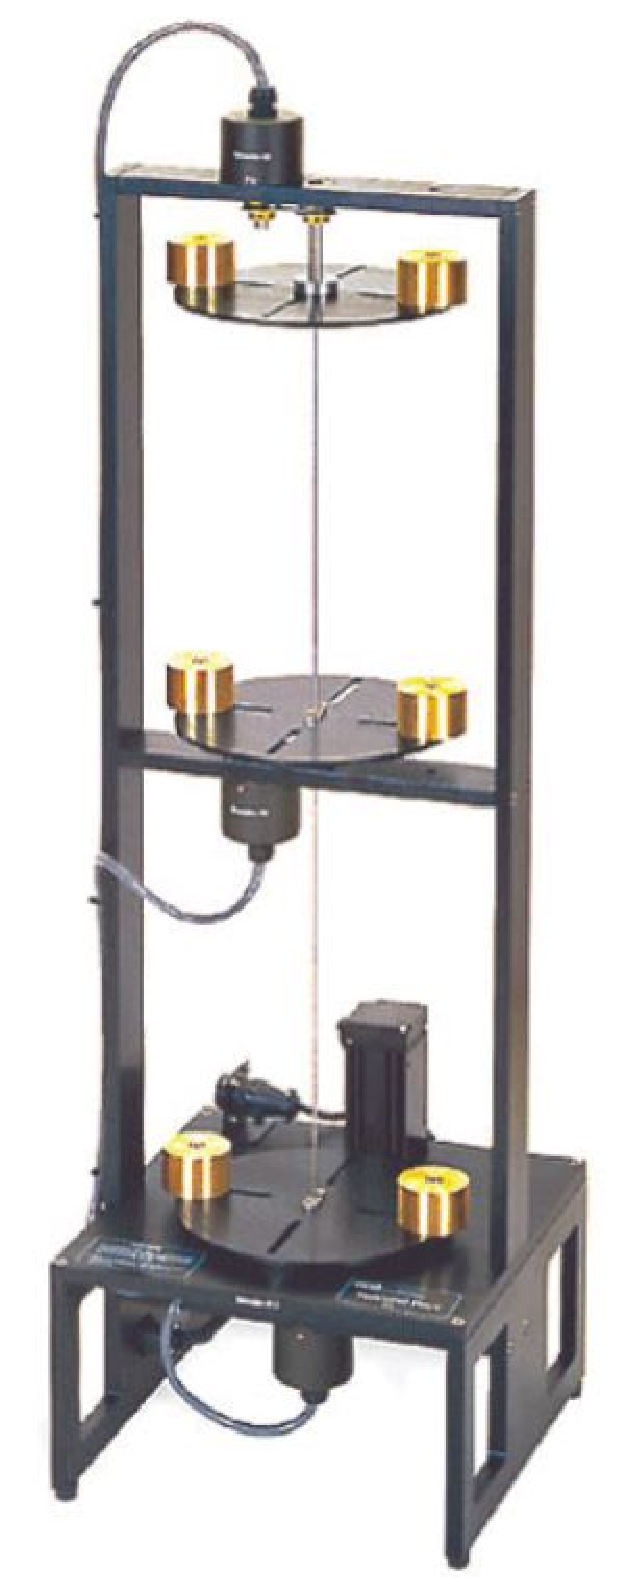
\includegraphics[scale=0.2]{pics/torsional_pic}
\caption{Torsional apparatus (ECP model 205a) used for the experimental analysis. The three disks are comprised of block masses which can be added or removed to alter the inertia of each disk (and thus alter the dynamics of the system). Each disk is vertically suspended on a spring with a variable spring constant. The actuator is located on the bottom of the device.}
\label{fig:torsional}
\end{figure}

\section{Experimental Analysis}
\label{sec:4}
In order to demonstrate the effectiveness of the proposed method, an RST controller will be designed for a multi-model torsional apparatus (ECP Model 205a), as shown in Fig.\ref{fig:torsional}. This system contains three disks with variable inertias suspended vertically on anti-friction ball bearings. The disks are connected through a non-rigid cable with an adjustable spring constant. The actuator (a high torque brushless motor with a $2$ Nm rating) is located at the bottom of the apparatus and is directly connected to the bottom disk via a rigid timing belt. The position of the disks are measured with a high resolution encoder ($16,000$ count/rev) and is used as feedback to control the closed-loop system. For this experiment, the dynamics of the apparatus will be altered by varying the inertias of the top disk. 

An RST controller will be designed for various inertial configurations. Three different configurations will be considered for this design; the bottom disk and the middle disk will possess fixed inertias, while the inertia for the top disk will be varied. The inertia is varied by altering the number of block masses that are arranged on the disk. 

The input to the system is the current of the actuator and the output is the position of the third disk. Therefore, the plant model has an integrator and is not stable; thus it is required to obtain the FRF's of the various configurations in a closed-loop structure. As asserted in Section (\ref{sec:21}), a stabilizing controller must be used to obtain $N(e^{-j\omega})$ and $M(e^{-j\omega})$. For this plant, a PID controller was designed to stabilize the closed-loop system. A reference input with a pseudo-random binary sequence (PRBS) is implemented to excite the closed-loop system with a sampling frequency of $25 \; Hz$. The time-domain signals for the reference input $r(t)$, control output $u(t)$, and output $y(t)$ for this system are depicted in Fig.\ref{fig:iddata} (for brevity, the figure shown is for one of the configurations). The FRF of $N(e^{-j\omega})$ is then obtained with the spectral analysis command in MATLAB (i.e., \texttt{spa($\cdot$)}) by using the time-domain data of $r(t)$ and $y(t)$. Similarly, the FRF of $M(e^{-j\omega})$ is obtained  in a similar fashion by using the time-domain data of $r(t)$ and $u(t)$. The FRF of the plant model can then be described as $G(e^{-j\omega}) = N(e^{-j\omega})M^{-1}(e^{-j\omega})$. The FRF's for each of the three configurations are shown in Fig.~\ref{fig:freq}.
\begin{figure}
\centering
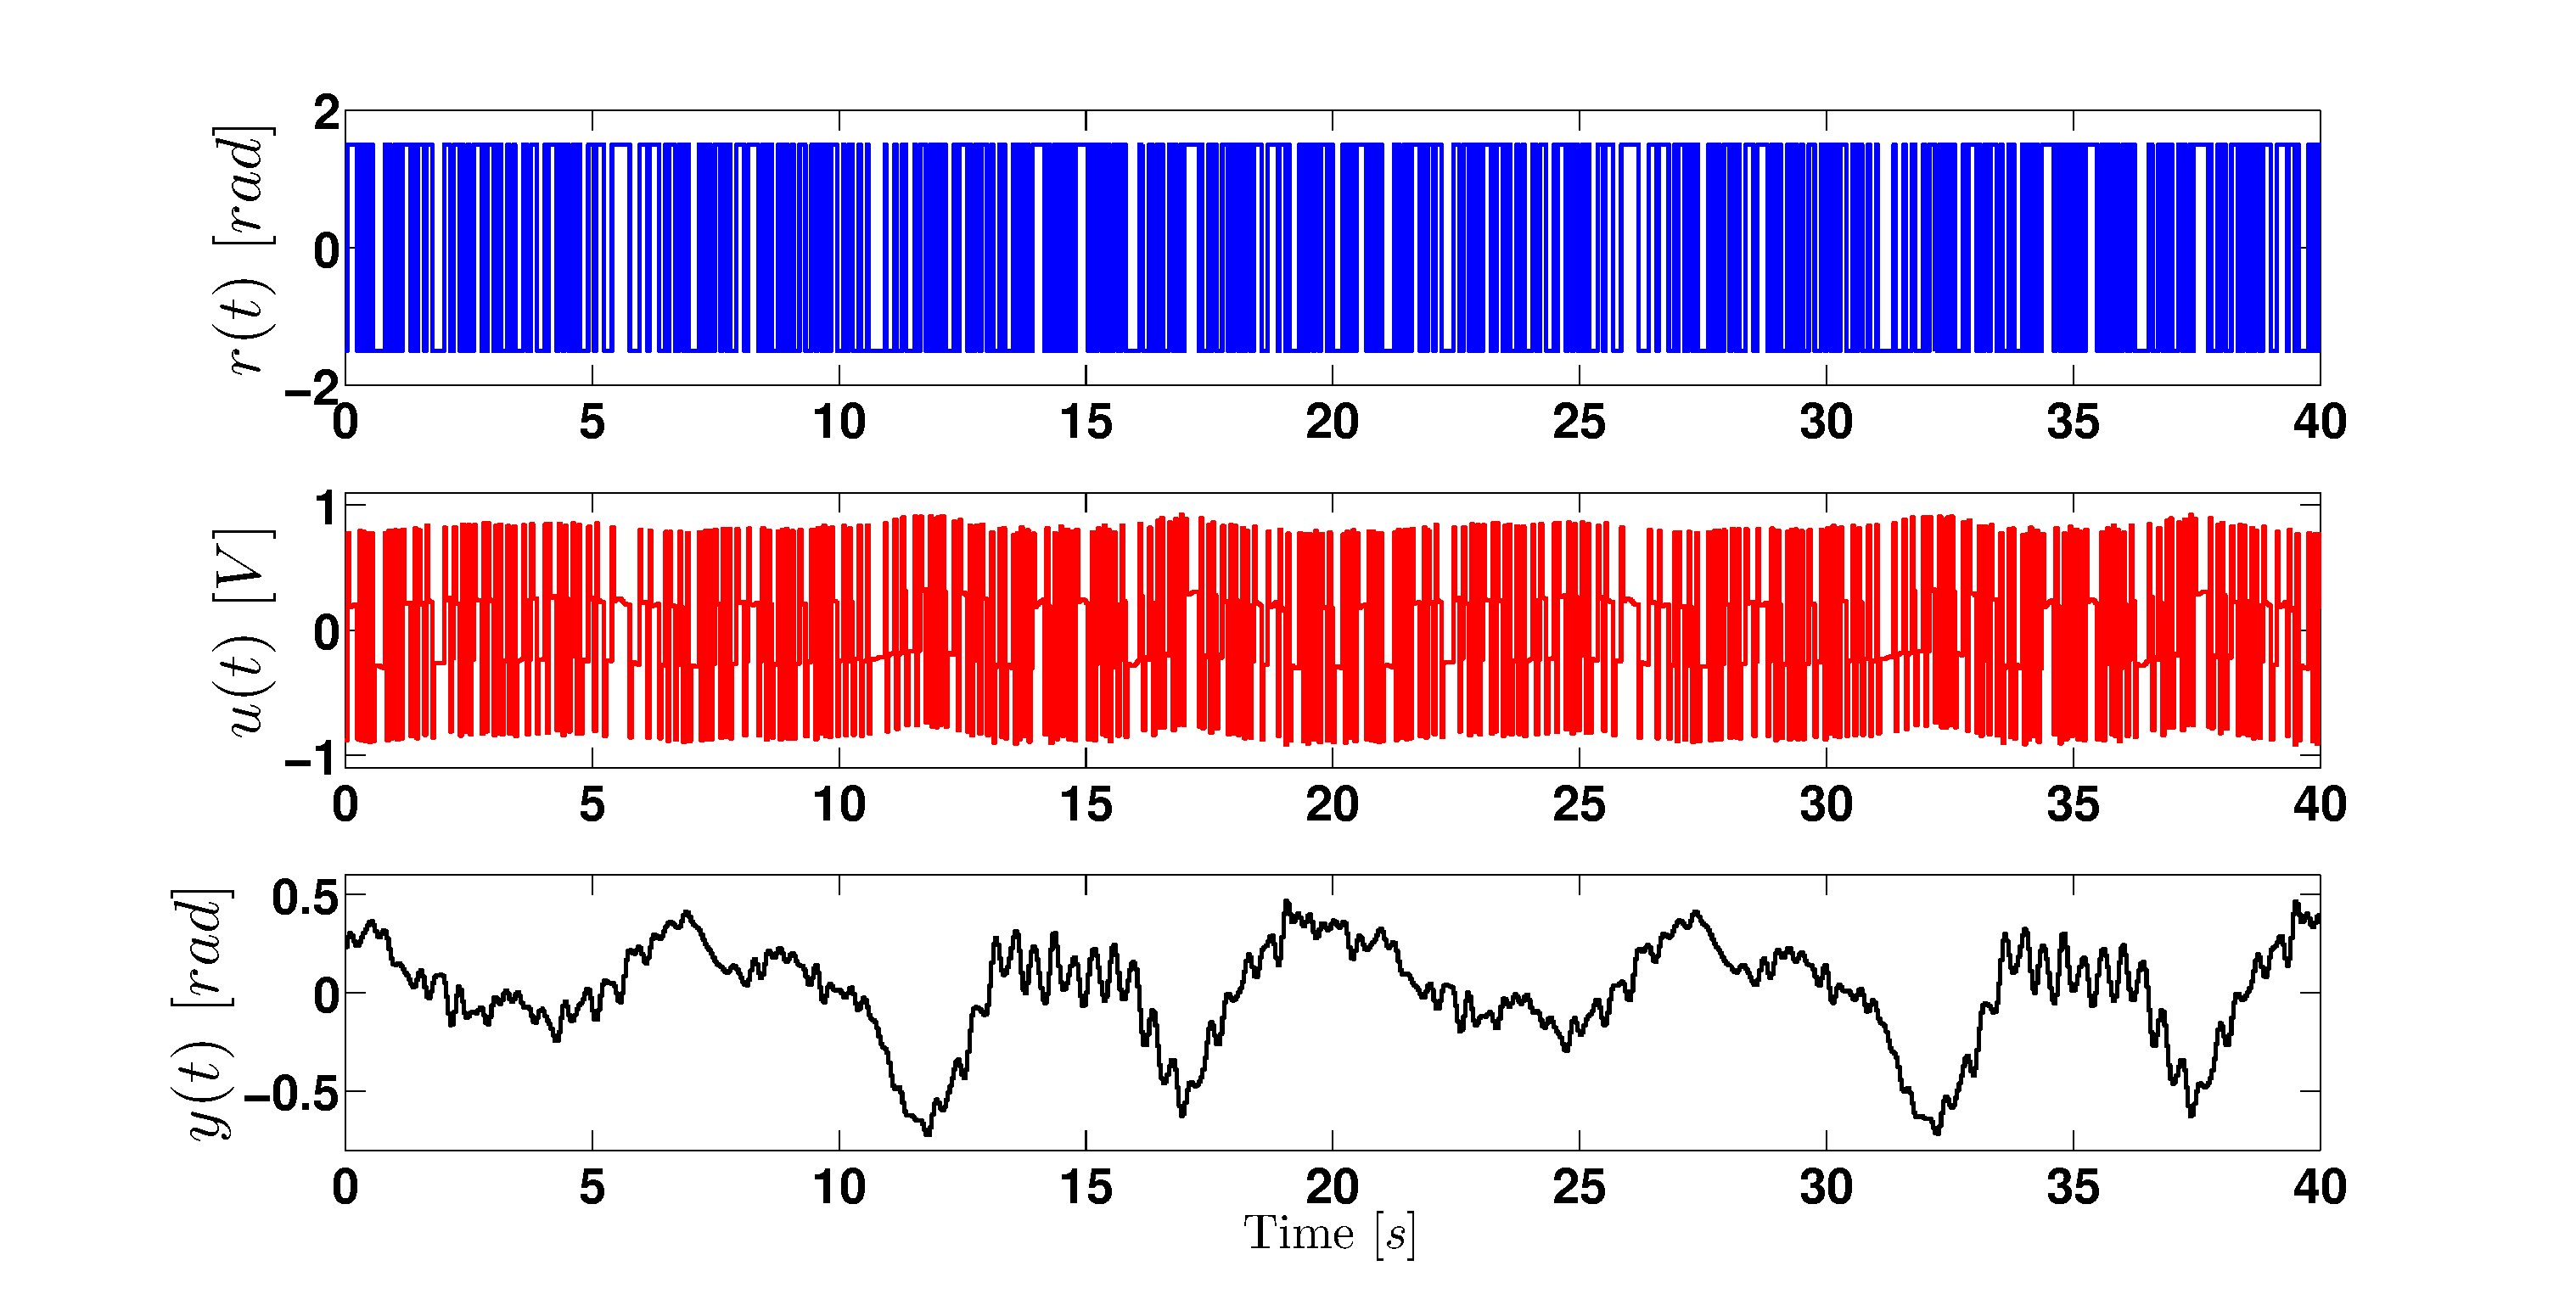
\includegraphics[width=1.1\columnwidth]{pics/id_data_2}
\caption{Time-domain response of the closed-loop system with a PRBS excitation signal (shown only for the system configuration with two block masses on the top disk): the PRBS reference input $r(t)$ with a register length of $511$ (solid-blue); control output $u(t)$ (solid-red); output response $y(t)$ (solid-black).}
\label{fig:iddata}
\end{figure}

\begin{figure}
\centering
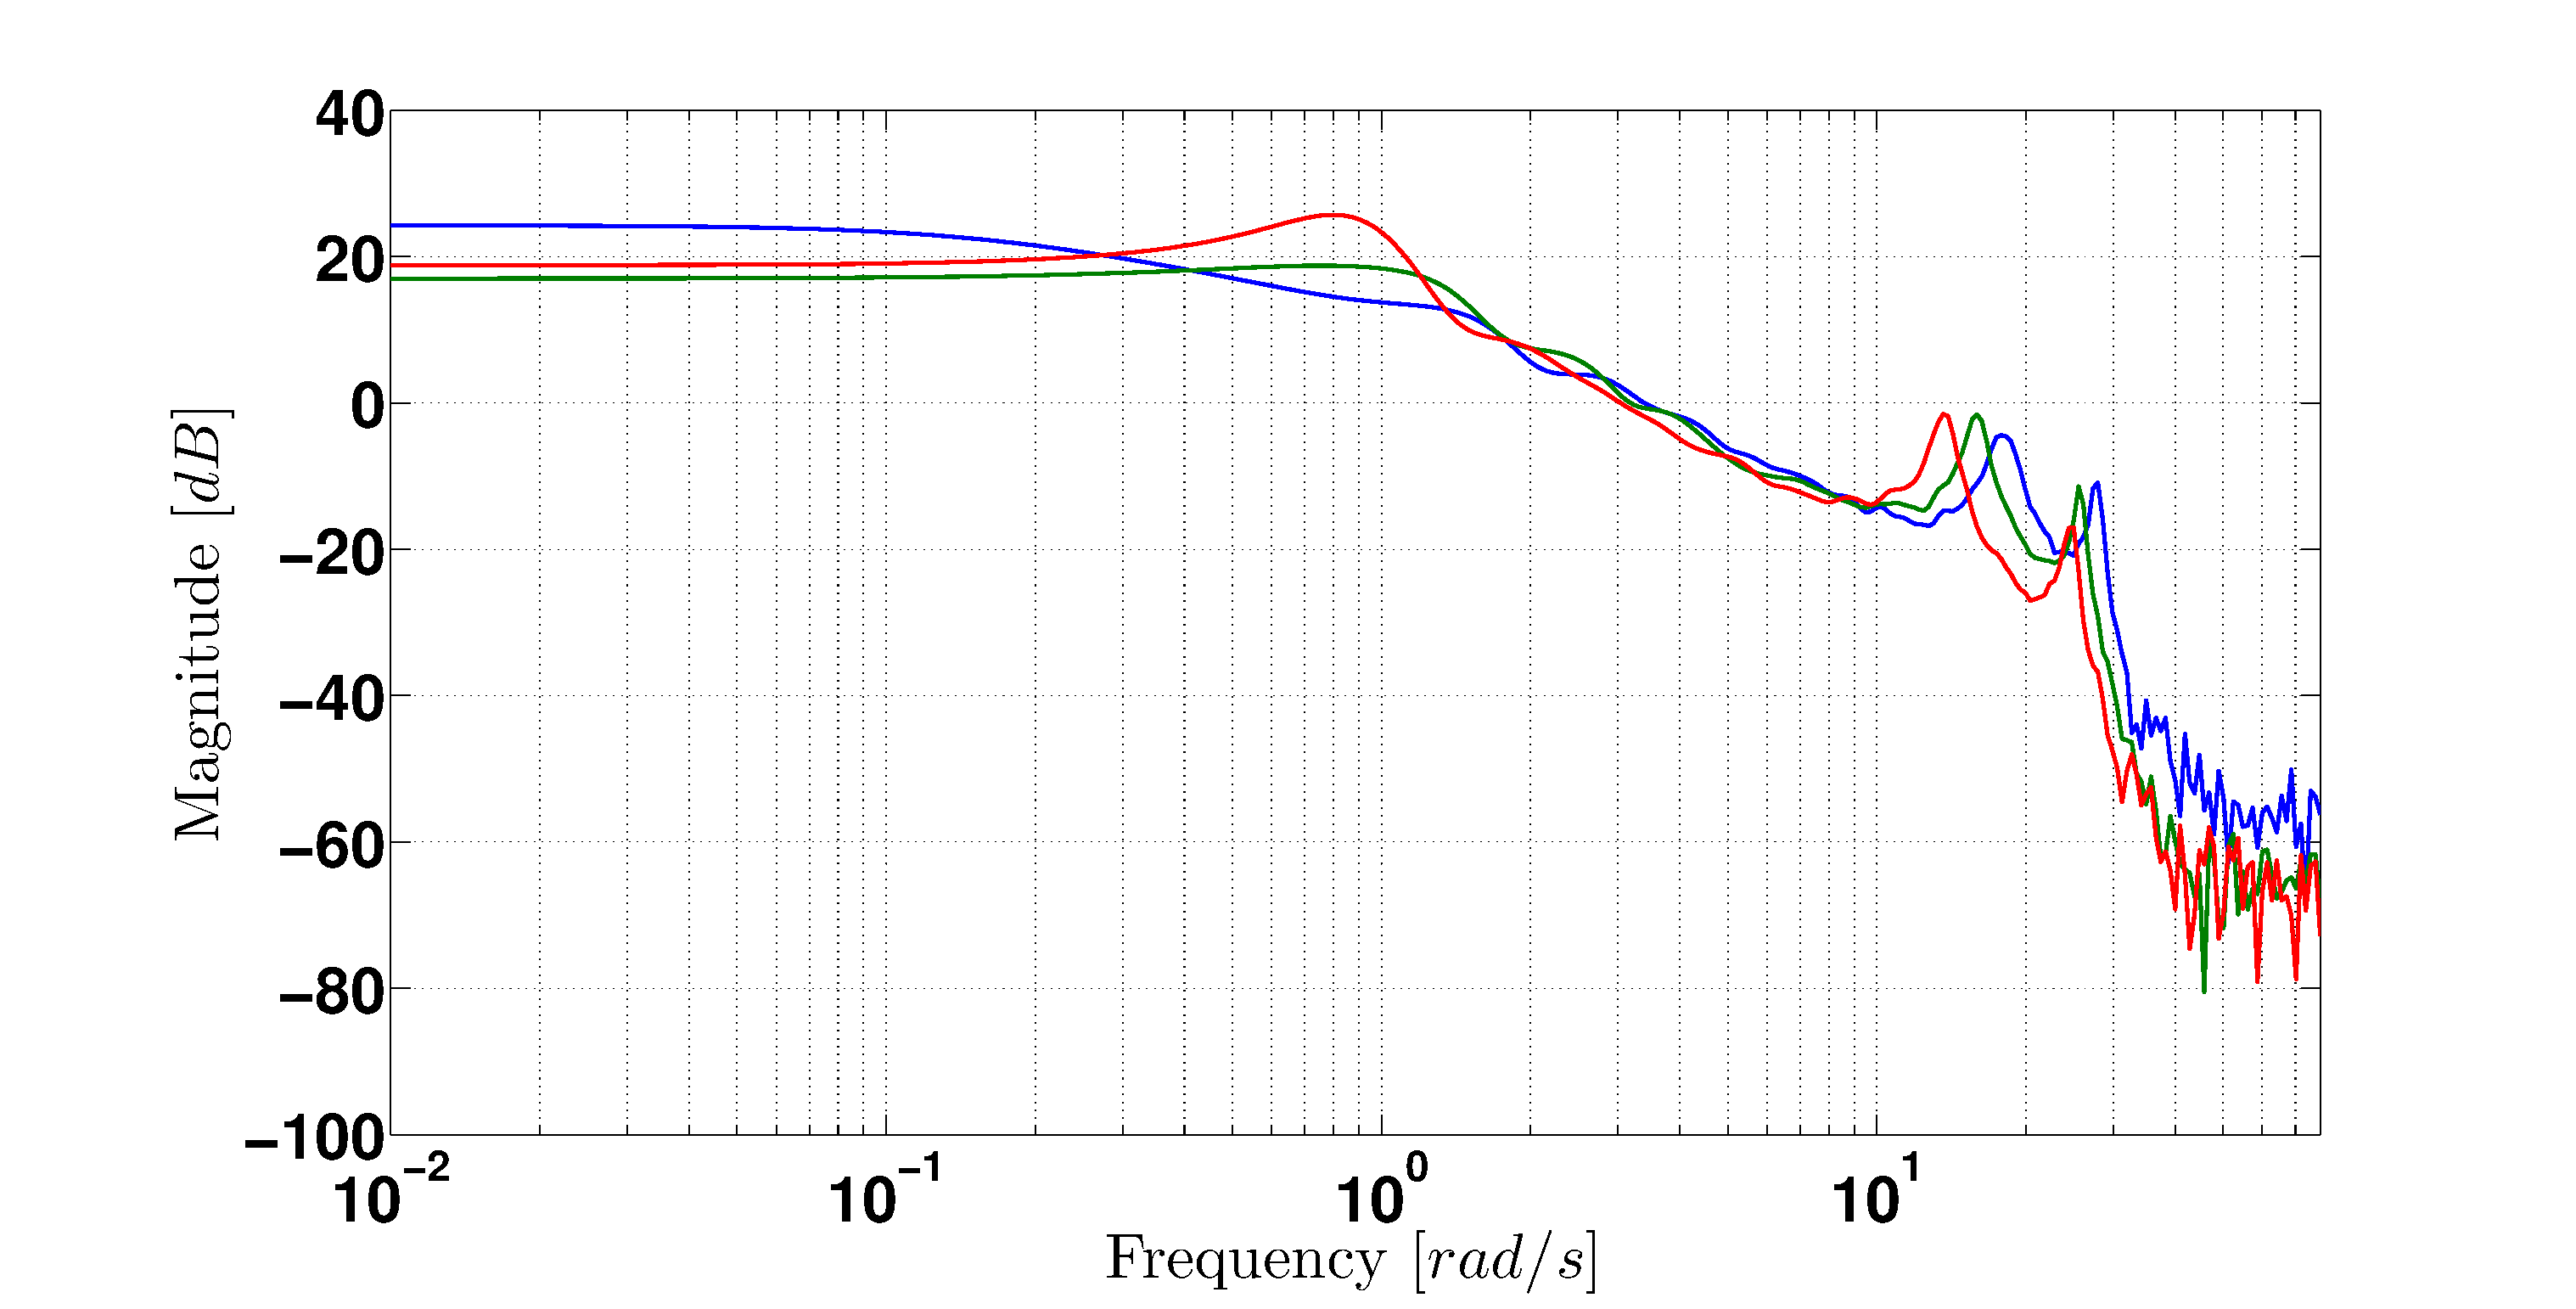
\includegraphics[width=\columnwidth]{pics/multi_freq_2}
\caption{FRF's of the plant model obtained from the closed-loop time-domain response of each system configuration. The loads on the bottom and middle disk are fixed while the load on the top disk is varied: FRF with one block mass on the top disk (solid-blue); FRF with two block masses on the top disk (solid-green); FRF with four block masses on the top disk (solid-red). }
\label{fig:freq}
\end{figure}


It will be desired to minimize the tracking error and to reject a step disturbance at the output. In order to achieve these specifications, an integrator will be included in $S^{\star}(z^{-1},\rho)$ (i.e., $S^{\star}(z^{-1},\rho) = (1-z^{-1})S(z^{-1},\rho)$). Additionally, a weight will be designated to limit the control effort. Therefore, the optimization problem formulated in (\ref{eq:min2}) will be implemented for this design scheme. The RST controllers will each be linearly parameterized as in (\ref{eq:Rc}), (\ref{eq:Sc}), (\ref{eq:Tc}) with $n_r = n_s = n_t = 8$. Thus the following optimization problem will be considered:
\iffalse
\begin{equation} \label{eq:min_exp}
\begin{aligned}
& \underset{ \{\rho_R,\rho_S,\rho_T\} \in \mathbb{R}}{\text{minimize}}
& & \gamma  \\
& \text{subject to:} & & \gamma^{-1} |W_2\jok[\psi_i^{\star}\jrok \\ & & &   \hspace{1.5cm} - N_i\jok T\jrok]|  \\ & & & \hspace{1.5cm} - \mathcal{R}e\{\psi_i^{\star}\jrok \}< 0  \\ 
& & & \gamma^{-1} |W_3\jok M_i\jok T\jrok|   \\ & & &   \hspace{1.5cm} - \mathcal{R}e\{\psi_i^{\star}\jrok \}< 0\\
& & & R(1,\rho) = T(1,\rho) \neq 0 \\
& & & \mbox{for }i = 1,2,3 \ \mbox{and }k = 1,\ldots,q
\end{aligned}
\end{equation}
where 
\begin{eqnarray*}
\psi_i^{\star}\jrok = M_i\jok S^{\star}\jrok \\ +N_i\jok R\jrok
\end{eqnarray*}
\fi
\begin{equation} \label{eq:min_exp}
\begin{aligned}
& \underset{ \{\rho_R,\rho_S,\rho_T\} \in \mathbb{R}}{\text{minimize}} \quad \gamma\\
& \text{subject to:} \\
& \gamma^{-1} |W_2\jok[\psi_i^{\star}\jrok - N_i\jok T\jrok]|  \\ & \hspace{4.2cm} - \mathcal{R}e\{\psi_i^{\star}\jrok \}< 0  \\
& \gamma^{-1} |W_3\jok M_i\jok T\jrok|   \\ & \hspace{4.2cm}  - \mathcal{R}e\{\psi_i^{\star}\jrok \}< 0 \\
& R(1,\rho) = T(1,\rho) \neq 0 \\
& \mbox{for }i = 1,2,3 \ \mbox{and }k = 1,\ldots,q
\end{aligned}
\end{equation}
where 
\begin{eqnarray*}
\psi_i^{\star}\jrok = M_i\jok S^{\star}\jrok \\ +N_i\jok R\jrok
\end{eqnarray*}

\subsection{Weighting filter selection}
The weighting filter $W_2$ will be chosen based on the fact that $\mathcal{E}_d + \mathcal{T}_d = 1$, where $\mathcal{E}_d$ is the desired error sensitivity function and $\mathcal{T}_d$ is the desired complementary sensitivity function (i.e., the closed-loop transfer function). $\mathcal{T}_d$ is chosen as a first order transfer function such that the step response will have a time constant of $1 \: s$ (which corresponds to a closed-loop bandwidth of $\omega_b = 1 \; rad/s$). The transfer function which satisfies these requirements can be formulated as
\begin{equation}
\mathcal{T}_d(s) = \frac{\omega_b}{s+\omega_b}
\end{equation}
Since $\mathcal{E}_d  = 1- \mathcal{T}_d$, an appropriate filter for the error sensitivity function can be devised as
\begin{equation}
W_2(s) = \frac{s+\omega_b}{s}
\end{equation}
It will be desired to minimize the control effort at high frequencies; therefore, a viable choice for the control weighting function $W_3$ is
\begin{equation}
W_3(s) = \frac{s + \omega_u / M_u}{\omega_u}
\end{equation}
where $M_u$ is the maximum controller gain, and $\omega_u$ is the controller bandwidth \cite{ZD98}. For the torsional system considered in this paper, an appropriate choice for these parameters are $M_u = 10^3$ and $\omega_u = 3 \; rad/s$. 
\subsection{Experimental results}
The optimization problem in (\ref{eq:min_exp}) is solved by considering a logarithmically spaced frequency grid with $q = 400$ points. The SDPT3 software package is used in conjunction with Matlab to solve the optimization problem. The solution obtained from the bisection algorithm produces the following controllers:

\begin{align*}
R(z^{-1}) &= 34.19 - 113.7 z^{-1} + 160  z^{-2} \\ &\qquad - 100.3 z^{-3} - 10.66 z^{-4} + 60.08 z^{-5} \\ &\qquad - 32.94 z^{-6} - 2.093 z^{-7} + 5.542 z^{-8}  \\
S^{\star}(z^{-1}) &=  1 + 0.3538 z^{-1} + 0.2304 z^{-2} - 0.07627 z^{-3} \\ &\qquad - 0.2845 z^{-4} - 0.2575 z^{-5} - 0.08136 z^{-6} \\ &\qquad - 0.1705 z^{-7} - 0.2921 z^{-8} - 0.422 z^{-9}\\
T(z^{-1}) &= 0.00942 + 0.01295 z^{-1} + 0.01548 z^{-2} \\ &\qquad + 0.01646  z^{-3} + 0.01116 z^{-4} + 0.01683 z^{-5} \\ &\qquad + 0.01491 z^{-6}  + 0.01329 z^{-7} + 0.01008 z^{-8}
\end{align*}

The optimal value of $\gamma$ obtained from the optimization is $\gamma_{opt} = 2.228$. The step responses obtained for each of the inertial configurations are depicted in Fig.~\ref{fig:step}. 
\begin{figure}
\centering
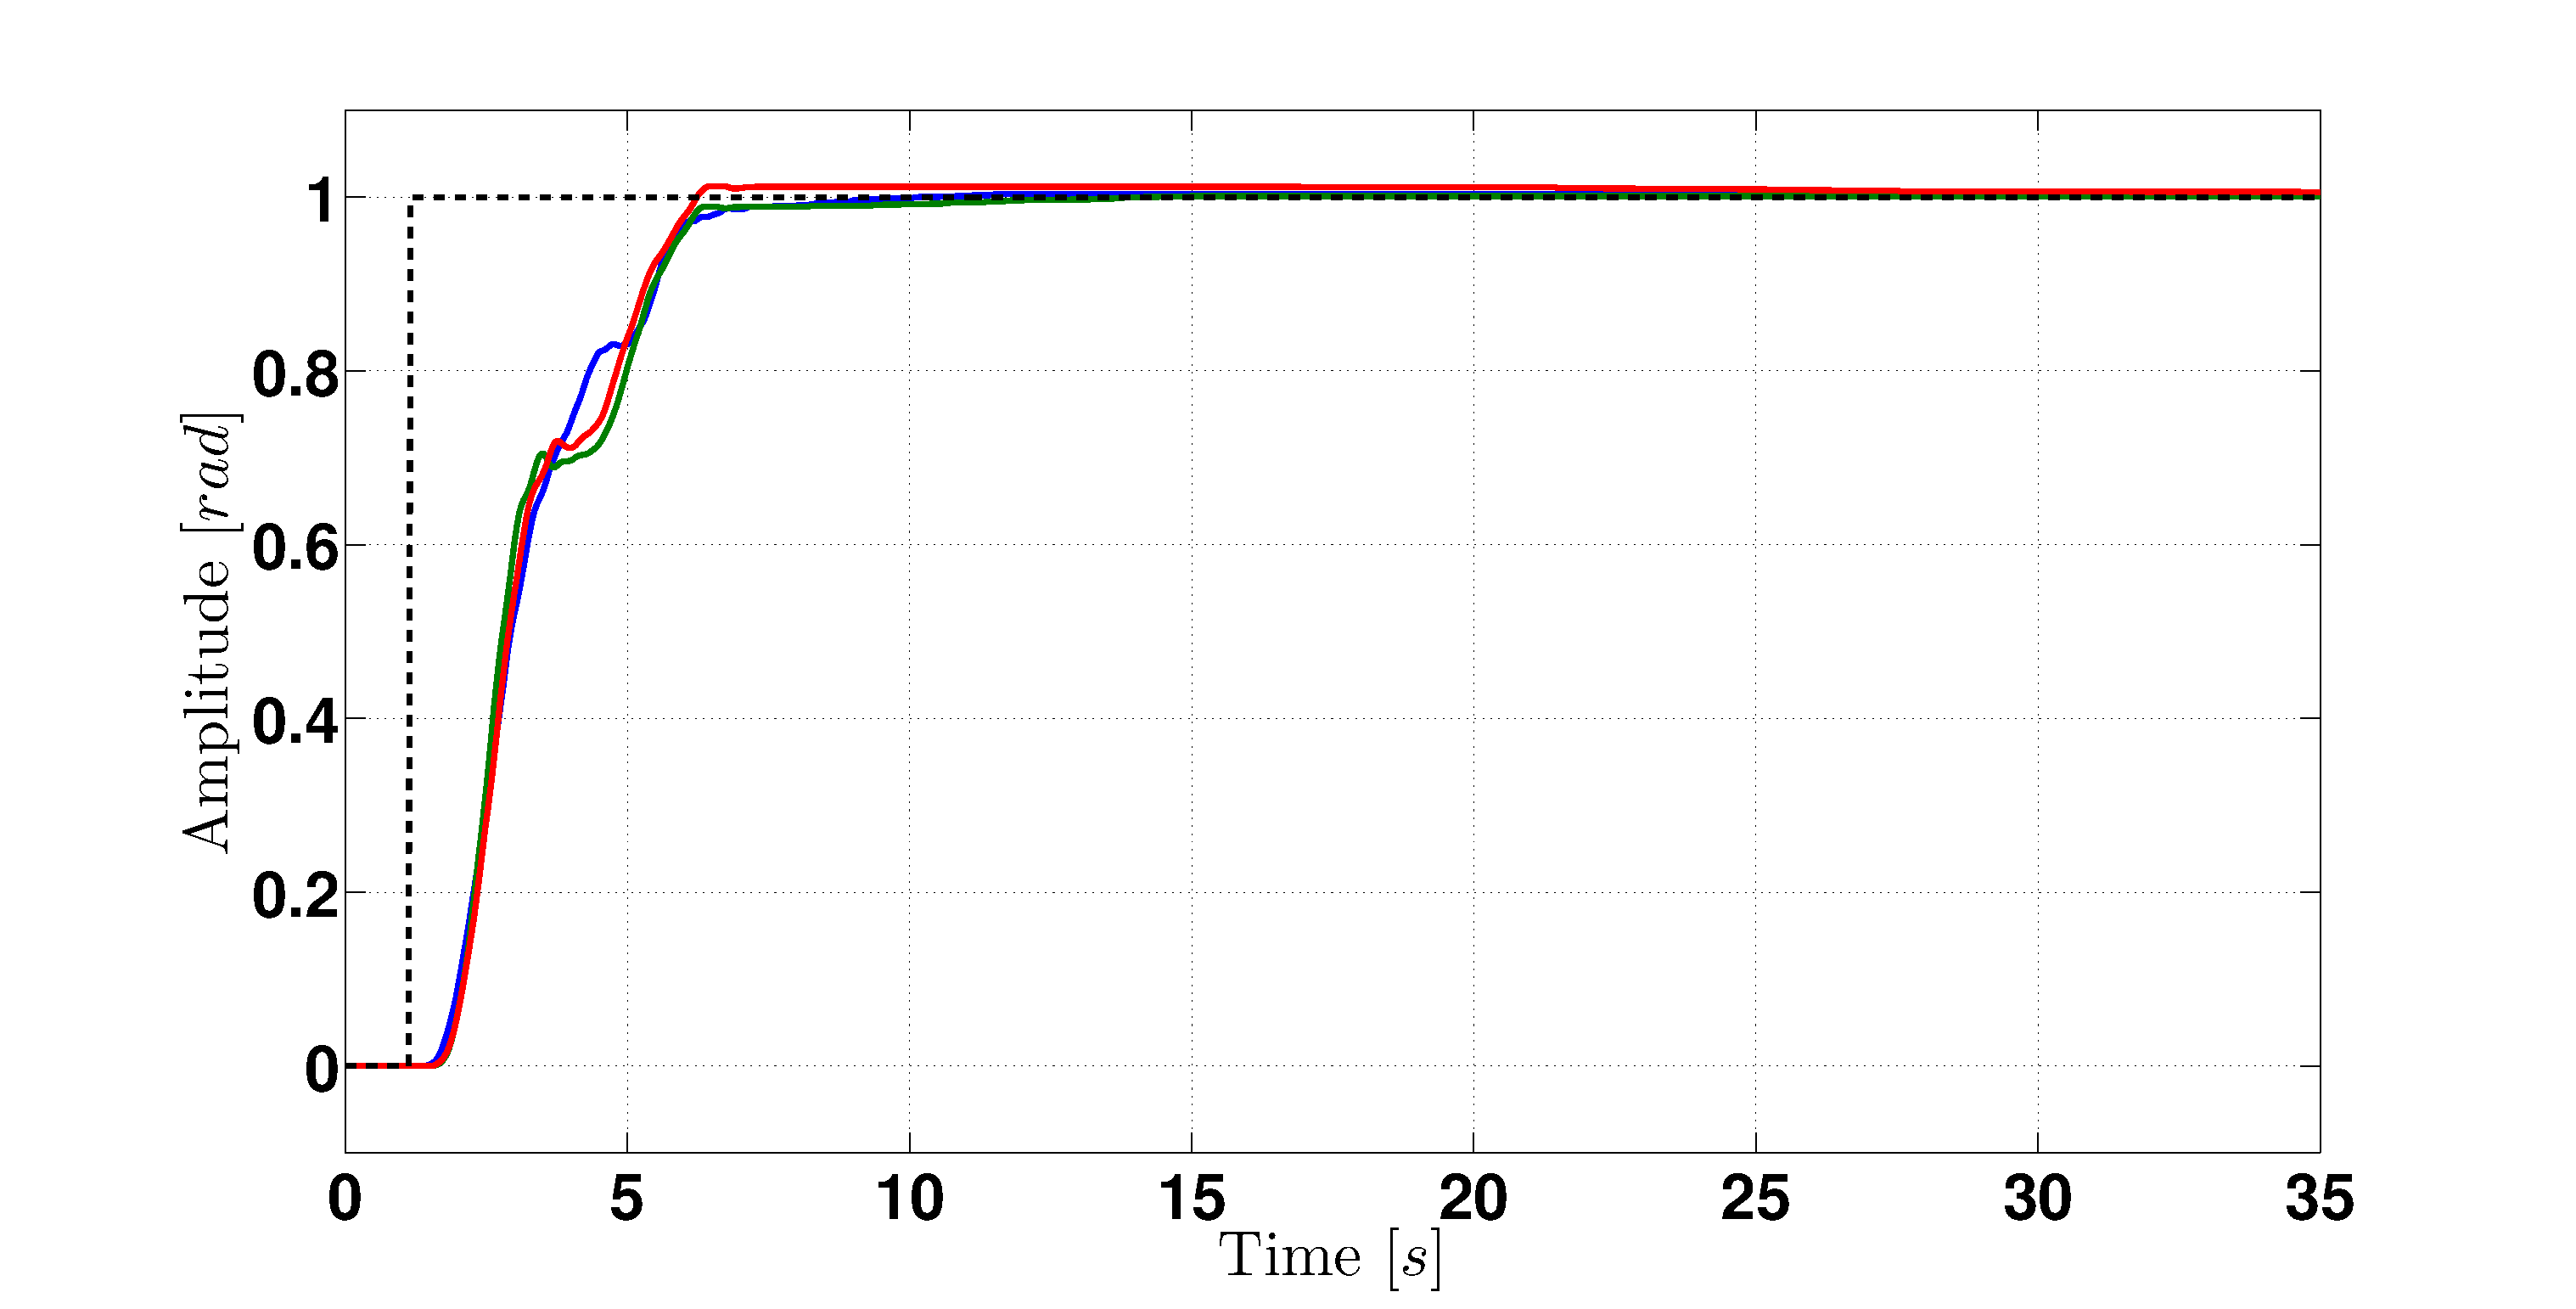
\includegraphics[width=\columnwidth]{pics/step_2}
\caption{Step response for each load configuration: response with one block mass on the top disk (solid-blue); response with two block masses on the top disk (solid-green); response with four block masses on the top disk (solid-red). }
\label{fig:step}
\end{figure}
From the multi-model step responses, it can be observed that the system is stable and robust to the dynamic variations of the torsional apparatus. Moreover, the load variations do not significantly impact the tracking performance (which is expected, since the same weighting filter was used in the multi-model optimization problem). The closed-loop FRF's of all three system configurations are shown in Fig.~\ref{fig:CL}. It can be observed that the achieved closed-loop bandwidth for all three configurations is approximately $1 \ rad/s$, which is the bandwidth that was specified to form the weighting filter $W_2(s)$. This confirms the feasibility of the solution obtained from the optimization problem in (\ref{eq:min_exp}).
\begin{figure}
\centering
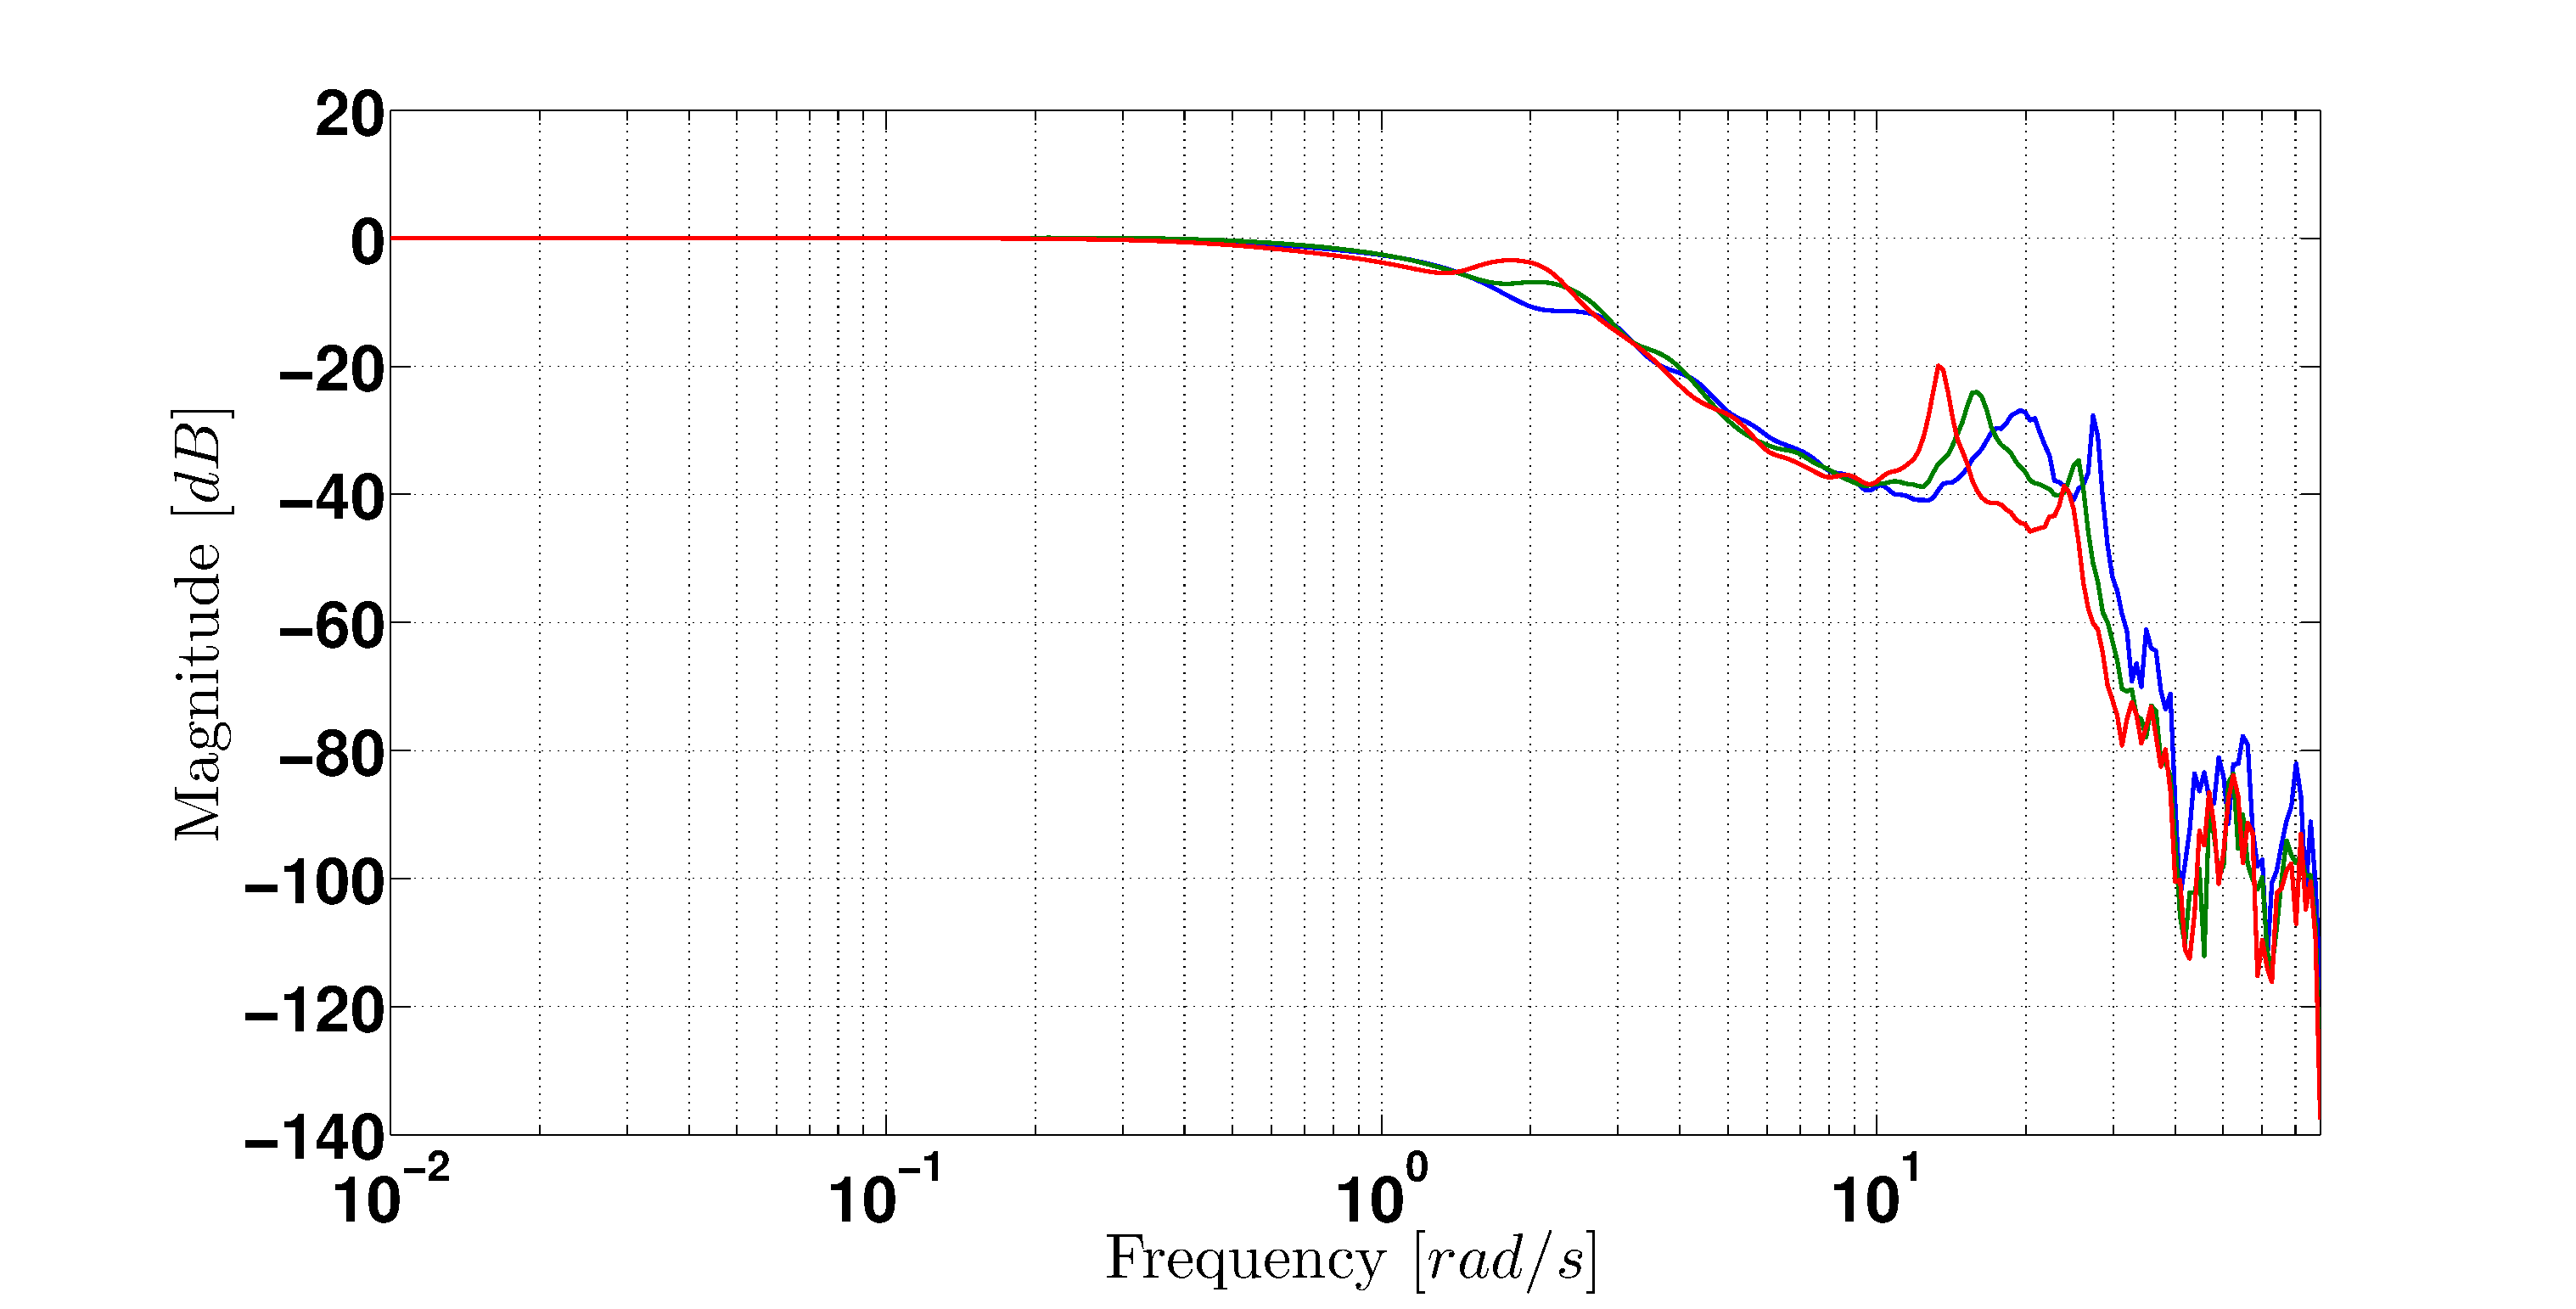
\includegraphics[width=\columnwidth]{pics/closed_loop}
\caption{Closed-loop frequency response functions of all three system configurations: closed-loop FRF with one block mass on the top disk (solid-blue); closed-loop FRF with two block masses on the top disk (solid-green); closed-loop FRF with four block masses on the top disk (solid-red).}
\label{fig:CL}
\end{figure}

\section{Conclusion}
\label{sec:5}
In this paper, a new method has been proposed to design robust controllers with $\mathcal{H}_{\infty}$ performance. The RST controller structure possesses many practical advantages, such as its two-degree of freedom design capabilities and the fact that it can be easily implemented. A frequency-domain approach has been used in order to avoid the problem of unmodeled dynamics associated with parametric models. A convex optimization problem is constructed based on the $\mathcal{H}_{\infty}$ criterion thanks to the process of linearly parameterizing the RST controllers. This controller design method has been employed to design a robust RST controller to control the disk position of a coupled torsional apparatus. A multi-model optimization approach was considered to design a controller for various loads; the design proved to be robust to the dynamic variations of the system. For further research, it will be desired to establish an optimal frequency gridding process, and compare how different gridding schemes can improve the solution to the optimization problem.



%\begin{IEEEbiographynophoto}
%Author1 Biography
%\end{IEEEbiographynophoto}
%\smallskip{}
%\begin{IEEEbiographynophoto}
%Author2 Biography
%\end{IEEEbiographynophoto}

\bibliography{linear}

\end{document}
